\documentclass{exam}

\usepackage{units} 
\usepackage{graphicx}
\usepackage[fleqn]{amsmath}
\usepackage{cancel}
\usepackage{float}
\usepackage{mdwlist}
\usepackage{booktabs}
\usepackage{cancel}
\usepackage{polynom}
\usepackage{caption}
\usepackage{fullpage}
\usepackage{xfrac}
\usepackage{enumerate}

\newcommand{\degree}{\ensuremath{^\circ}} 
\everymath{\displaystyle}

% \begin{figure}[H]
%   \centering
%   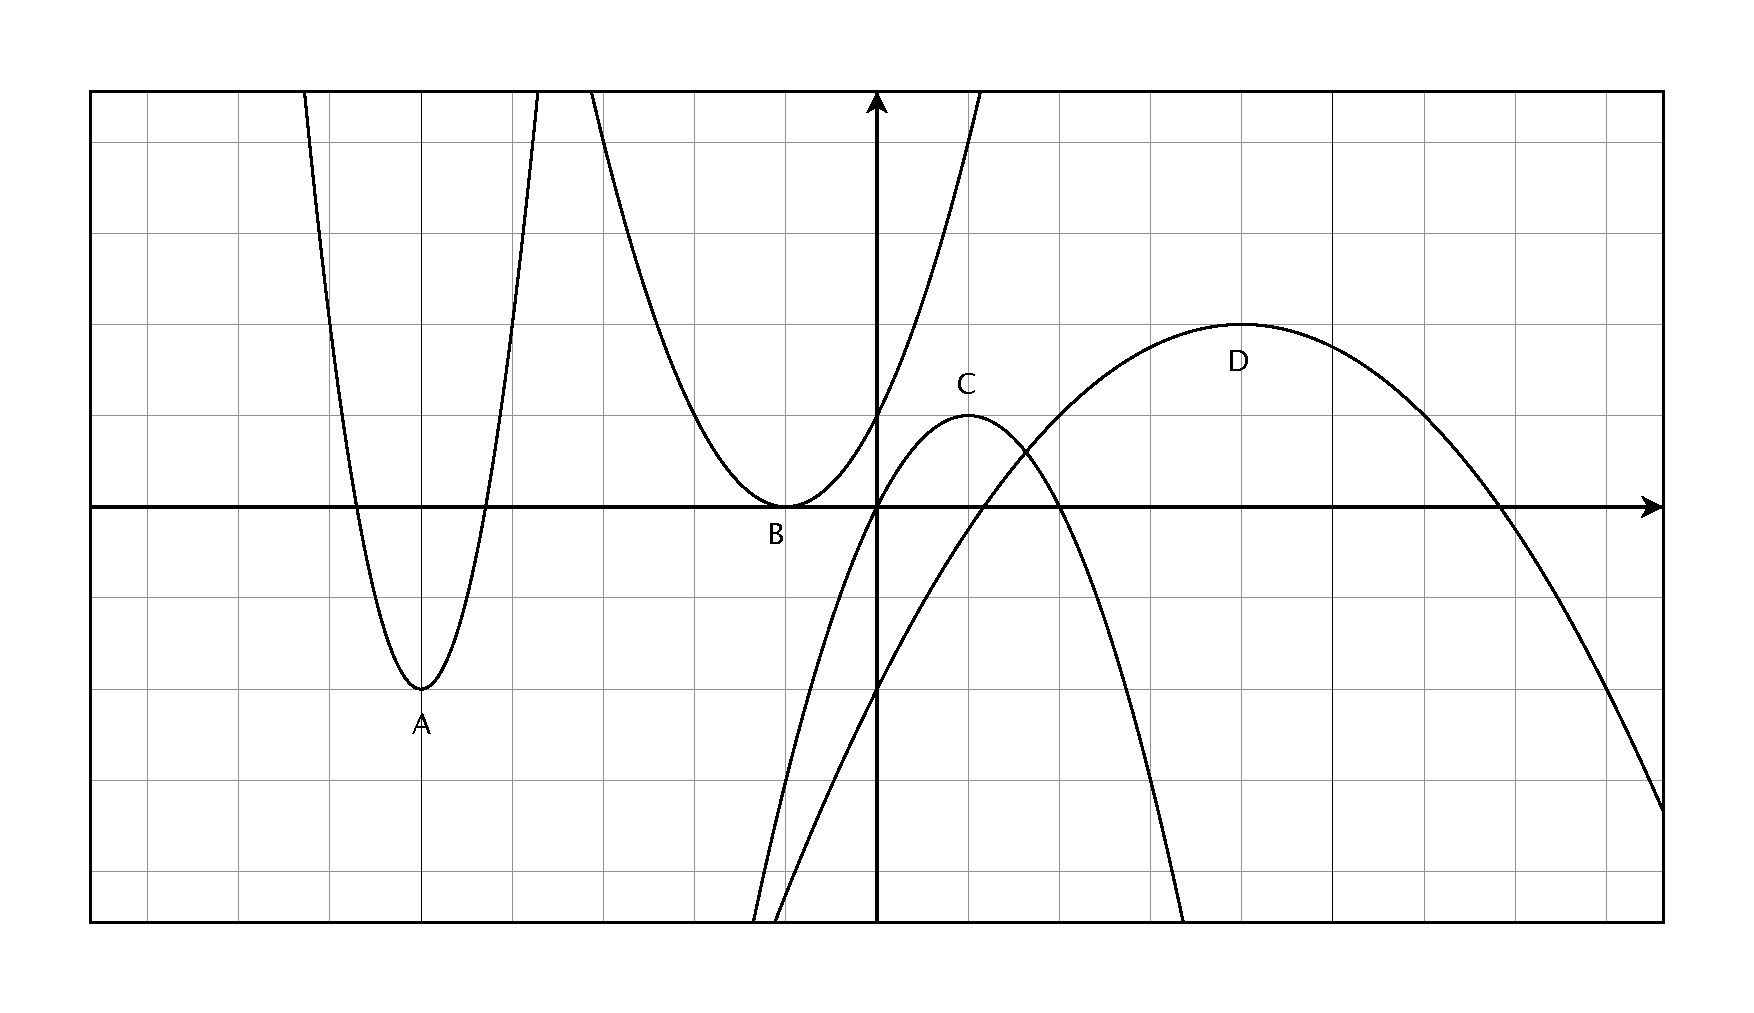
\includegraphics[scale=.3]{problem_7.eps}
%   \caption*{Problem 7}
% \end{figure}

% \begin{tabular}{cc}
% \toprule
% period & amplitude \\
% \midrule
%   $\pi$ & $2$ \\
% \bottomrule
% \end{tabular}

\printanswers

\ifprintanswers 
  \usepackage{2in1, lscape} 
\fi

\date{February 27, 2013}
\title{Math 141 \\ Homework 5}

\begin{document}

\maketitle

\section{Homework}

\begin{itemize*}
  \item Read Section 2.7
  \item Section 2.6: 6-11, 15-16, 24, 27
  \item Section 2.7: 1-10, 17-26, 30-31, 34-35, 40-42, 45-52, 57, 59, 60
\end{itemize*}

\ifprintanswers
  \pagebreak
\fi

\section{Extra Credit}
\begin{itemize}
  \item A boat leaves a dock at 2:00 PM and travels due south at \unit[20]{km/hr}.  Another boat has been heading due
    east at \unit[15]{km/hr} and reaches the same dock at 3:00 PM.  At what time were the two boats closest together?

    \begin{solution}
      The southbound boat starts at port and heads off in the negative y direction, so its distance is given by:
      \[
        y(t) = 20t
      \]

      At 2:00 when the southbound boat started, the eastbound boat was an hour, or \unit[15]{km} away from port.  This
      means the distance from port for the eastbound boat is:
      \[
        x(t) = 15 - 15t
      \]

      The square of the distance between the two boats is:
      \begin{align*}
        d(t) &= x^2 + y^2 \\
             &= (15 - 15t)^2 + (20t)^2 \\
             &= 225 - 450t + 225t^2 + 400t^2 \\
             &= 625t^2 - 450t - 225 \\
      \end{align*}

      The shortest distance occurs at:
      \begin{align*}
        t &= \frac{450}{2 \cdot 625} \\
          &= \unit[0.36]{hour} \\
      \end{align*}

      0.36 hours after 2:00 is about 2:22.

    \end{solution}

  \ifprintanswers
    \pagebreak
  \fi

  \item Section 2.7, problems 64-65
    \begin{solution}
      \begin{description}

        \item[64]
          \begin{align*}
            (f \circ g)(x) &= m_1 (m_2x + b_2) + b_1 \\
              &= m_1m_2x + m_1b_2 + b_1 \\
          \end{align*}

          The composition is a line with slope $m_1m_2$ and y-intercept $m_1b_2 + b_1$.

        \item[65]
          \begin{parts}
            \part
              Squaring $g(x)$ and adding 6 produces $h(x)$, so the function $f(x)$ should be:
              \[
                f(x) = x^2 + 6
              \]
              With this $f$: 
              \begin{align*}
                (f \circ g)(x) &= (2x + 1)^2 + 6 \\
                  &= 4x^2 + 4x + 7 \\
                  &= h(x)
              \end{align*}
            
            \part If $g(x) = x^2 + x - 1$, then 
            \begin{align*}
              (f \circ g)(x) &= 3(x^2 + x - 1) + 5 \\
                &= 3x^2 + 3x + 2 \\
                &= h(x)
            \end{align*}
              
          \end{parts}
      \end{description}
    \end{solution}
\end{itemize}

\ifprintanswers
  \pagebreak

  \section{Section 2.6}
  \begin{description}
    \item[6] 
      If we call the sides $x$ and $y$, we can find an expression for one side in terms of the area and the other
      side:
      \begin{align*}
        A &= xy \\
        16 &= xy \\
        y &= \frac{16}{x} \\
      \end{align*}

      Now we can find the function for the perimeter:
      \begin{align*}
        P    &= 2x + 2y \\
        P(x) &= 2x + \frac{32}{x} \\
      \end{align*}

    \item[7]
      The formula for the area of a triangle is $A = \dfrac{1}{2} bh$.  The missing piece is the height, but we can use
      the Pythagorean theorem to find it:
      \begin{align*}
        \left( \frac{x}{2} \right)^2 + h^2 &= x^2 \\
        \frac{x^2}{4} + h^2                &= x^2 \\
        h^2                                &= \frac{3x^2}{4} \\
        h                                  &= \frac{\sqrt{3}}{2} x \\
      \end{align*}

      Now we can find a function for the area in terms of the side length:
      \begin{align*}
        A(x) &= \frac{1}{2} x \cdot \frac{\sqrt{3}}{2} x  \\
             &= \frac{\sqrt{3}}{4} x^2 \\
      \end{align*}

    \item[8]
      The formulas for surface area and volume in terms of side length are:
      \begin{align*}
        A &= 6x^2 \\
        V &= x^3 \\
      \end{align*}

      To find a function for the area in terms of the volume, we need to solve the volume equation for $x$: 
      \[
        x = \sqrt[3]{V} = V^{1/3}
      \]
      
      Now we can find area as a function of the volume:
      \[
        A(V) = 6(V^{1/3})^2 = 6 V^{2/3}
      \]

    \item[9]
      \begin{align*}
        A    &= \pi r^2 \\
        r(A) &= \sqrt{\frac{A}{\pi}} \\
      \end{align*}

    \item[10]
      Solve the circumference equation for $r$:
      \begin{align*}
        C &= 2 \pi r \\
        r &= \frac{C}{2 \pi} \\
      \end{align*}

      Find the function for the area:
      \begin{align*}
        A    &= \pi r^2 \\
        A(C) &= \pi \cdot \left( \frac{C}{2 \pi} \right)^2 \\
             &= \frac{C^2}{4 \pi} \\
      \end{align*}

    \item[11]
      If the length of a side is $x$ and the height is $h$:
      \begin{align*}
        V &= x^2h \\
        S &= 2x^2 + 4xh \\
      \end{align*}

      Since the volume is fixed at 60, we can solve the volume equation for $h$ to get a surface area equation that just
      contains $x$:
      \begin{align*}
        h    &= \frac{60}{x^2} \\
        S(x) &= 2x^2 + \frac{240}{x} \\
      \end{align*}

    \item[15]
      If we call the length of the two equal sides $s$:
      \begin{align*}
        8 &= 2s + b \\
        s &= 4 - \frac{b}{2} \\
      \end{align*}

      To find the area, we need the height:
      \begin{align*}
        \left( \frac{b}{2} \right)^2 + h^2 &= s^2 \\
        h                                  &= \sqrt{s^2 - \frac{b^2}{4}} \\
      \end{align*}

      If we plug the expression for $s$, we can get the height in terms of the base:

      \begin{align*}
        h &= \sqrt{\left( 4 - \frac{b}{2} \right)^2 - \frac{b^2}{4}} \\
          &= \sqrt{16 - 4b} \\
          &= 2 \sqrt{4 - b} \\
      \end{align*}

      The area is
      \begin{align*}
        A &= \frac{1}{2} bh \\
          &= \frac{1}{2} b \cdot (2 \sqrt{4 - b}) \\
          &= b \sqrt{4 - b} \\
      \end{align*}

    \item[16]
      If the length of the shortest side is $a$, the length of the next longest side is $2a$ and the length of the
      hypotenuse is:
      \[
        \sqrt{a^2 + (2a)^2} = \sqrt{5a^2} = a \sqrt{5}
      \]

      The perimeter length is the sum of all the side lengths:
      \[
        P(a) = 2a + a + a \sqrt{5} = 3a + a \sqrt{5} = a(3 + \sqrt{5})
      \]

    \item[24]
      If one side of the pen is $x$ and the other side is $y$, the perimeter is:
      \[
        P = 5x + 2y \\
      \]

      We want a function in terms of one of the variables, so we can solve the perimeter equation for one of the sides:
      \begin{align*}
        750 &= 5x + 2y \\
        2y  &= 750 - 5x \\
        y   &= 375 - \frac{5x}{2} \\
      \end{align*}

      The area function is: 
      \begin{align*}
        A    &= xy \\
        A(x) &= x \left( 375 - \frac{5x}{2} \right) \\
             &= -\frac{5x^2}{2} + 375x \\
      \end{align*}

      Find the maximum:
      \begin{align*}
        A(x) &= \frac{-375}{-5} \\        
             &= 75 \\        
      \end{align*}

      Plug back in to find $y$:
      \[
        y = 375 - \frac{5 \cdot 75}{2} = 187.5
      \]
      The largest area pen has dimensions 75 ft by 187.5 ft which provides an area of $\unit{14,062.5}{ft^2}$.

    \item[27]
      \begin{parts}
        \part
          First, find an equation for the number of spectators in terms of the ticket price:
          \[
            S(p) = 27,000 + 3,000(10 - p) = 57,000 - 3,000p
          \]

          The revenue is the number of spectators multiplied by the ticket price:
          \[
            R(p) = -3,000p^2 + 57,000p 
          \]

        \part
          Set the revenue to zero and solve for $p$:
          \begin{align*}
            57,000p - 3,000p^2 &= 0 \\
            3,000p(19 - p)     &= 0 \\
            p                  &= \left\{ 0, 19 \right\} \\
          \end{align*}
          With a ticket price of \$0 there are plenty of fans, but there isn't any revenue.  With a ticket price of \$19,
          there aren't any fans.

        \part
          \begin{align*}
            p_{max} &= \frac{-57,000}{-6,000} \\
                    &= 9.5 \\
          \end{align*}

          The best price to charge is \$9.50.  This gives a total revenue of \$270,750 by bringing in 28,500 fans.
      \end{parts}
  \end{description}

  \pagebreak

  \section{Section 2.7}

  \begin{description}

    \item[1] 
      \begin{tabular}{lr}
        \toprule
        function & domain \\
        \midrule
        $(f + g)(x) = x^2 + x - 3$     & $(-\infty, \infty)$ \\
        \midrule
        $(f - g)(x) = -x^2 + x - 3$    & $(-\infty, \infty)$ \\
        \midrule
        $(fg)(x) = x^2(x - 3)$         & $(-\infty, \infty)$ \\
        \midrule
        $(f/g)(x) = \frac{x - 3}{x^2}$ & $x \neq 0$ \\
        \bottomrule
      \end{tabular}

    \item[2] 
      \begin{tabular}{lr}
        \toprule
        function & domain \\
        \midrule
        $(f + g)(x) = 4x^2 + 2x - 1$       & $(-\infty, \infty)$ \\
        \midrule
        $(f - g)(x) = -2x^2 + 2x + 1$      & $(-\infty, \infty)$ \\
        \midrule
        $(fg)(x) = 3x^4 + 6x^3 - x^2 - 2x$ & $(-\infty, \infty)$ \\
        \midrule
        $(f/g)(x) = \frac{x^2 + 2x}{3x^2 - 1}$ & $x \neq \pm \frac{\sqrt{3}}{3}$ \\
        \bottomrule
      \end{tabular}

    \item[3] 
      \begin{tabular}{lr}
        \toprule
        function & domain \\
        \midrule
        $(f + g)(x) = \sqrt{4 - x^2} + \sqrt{1 + x}$ & $[-1, 2]$ \\
        \midrule
        $(f - g)(x) = \sqrt{4 - x^2} - \sqrt{1 + x}$ & $[-1, 2]$ \\
        \midrule
        $(fg)(x)  = \sqrt{-x^3 - x^2 + 4x + 4}$      & $[-1, 2]$ \\
        \midrule
        $(f/g)(x) = \sqrt{ \frac{4 - x^2}{1 + x} }$  & $(-1, 2]$ \\    
        \bottomrule
      \end{tabular}

    \item[4] 
      \begin{tabular}{lr}
        \toprule
        function & domain \\
        \midrule
        $(f + g)(x) = \sqrt{9 - x^2} + \sqrt{x^2 - 4}$  & $[-3, -2] \cup [2, 3]$ \\
        \midrule
        $(f - g)(x) = \sqrt{9 - x^2} - \sqrt{x^2 - 4}$  & $[-3, -2] \cup [2, 3]$ \\
        \midrule
        $(fg)(x)    = \sqrt{-x^4 + 13x^2 - 36}$         & $[-3, -2] \cup [2, 3]$ \\
        \midrule
        $(f/g)(x)   = \sqrt{ \frac{9 - x^2}{x^2 - 4} }$ & $[-3, -2) \cup (2, 3]$ \\
        \bottomrule
      \end{tabular}

    \item[5] 
      \begin{tabular}{lr}
        \toprule
        function & domain \\
        \midrule
        $(f + g)(x) = \frac{2}{x} + \frac{4}{x + 4} = \frac{6x + 8}{x^2 + 4x}$  & $x \neq \{-4, 0\}$ \\
        \midrule
        $(f - g)(x) = \frac{2}{x} - \frac{4}{x + 4} = \frac{-2x + 8}{x^2 + 4x}$ & $x \neq \{-4, 0\}$ \\
        \midrule
        $(fg)(x)  = \frac{8}{x^2 + 4x}$ & $x \neq \{-4, 0\}$ \\
        \midrule
        $(f/g)(x) = \frac{x + 4}{2x}$   & $x \neq \{-4, 0\}$ \\
        \bottomrule
      \end{tabular}

    \item[6] 
      \begin{tabular}{lr}
        \toprule
        function & domain \\
        \midrule
        $(f + g)(x) = \frac{2 + x}{x + 1}$  & $x \neq -1$ \\
        \midrule
        $(f - g)(x) = \frac{2 - x}{x + 1}$  & $x \neq -1$ \\
        \midrule
        $(fg)(x)    = \frac{2x}{(x + 1)^2}$ & $x \neq -1$ \\
        \midrule
        $(f/g)(x)   = \frac{2}{x}$          & $x \neq \{-1, 0\}$ \\
        \bottomrule
      \end{tabular}

    \item[7] $[0, 1]$

    \item[8] $[-1, 0) \cup (0, \infty)$

    \item[9]
      \[
        (x - 3)^{-1/4} = \frac{1}{\sqrt[4]{x - 3}}
      \]
      So the domain is: $(3, \infty)$.

    \item[10] $[-3, 1) \cup (1, \infty)$

\pagebreak

    \item[17]
      \begin{parts}

        \part
          \begin{align*}
            g(0)    &= 2 \\
            f(2)    &= 1 \\
            \\
            f(g(0)) &= 1 \\
          \end{align*}

        \part
          \begin{align*}
            f(0)    &= -5 \\
            g(-5)   &= -23 \\
            \\
            g(f(0)) &= -23 \\
          \end{align*}

      \end{parts}

    \item[18]
      \begin{parts}

        \part
          \begin{align*}
            f(4)    &= 7 \\
            f(7)    &= 16 \\
            \\
            f(f(4)) &= 16 \\
          \end{align*}

        \part
          \begin{align*}
            g(3)    &= -7 \\
            g(-7)   &= -47 \\
            \\
            g(g(3)) &= -47 \\
          \end{align*}

      \end{parts}

    \item[19]
      \begin{parts}

        \part
          \begin{align*}
            g(-2)           &= -2 \\
            f(-2)           &= -11 \\
            \\
            (f \circ g)(-2) &= -11 \\
          \end{align*}

        \part
          \begin{align*}
            f(-2)           &= -11 \\
            g(-11)          &= -119 \\
            \\
            (g \circ f)(-2) &= -119 \\
          \end{align*}

      \end{parts}

    \item[20]
      \begin{parts}

        \part
          \begin{align*}
            f(-1)           &= -8 \\
            f(-8)           &= -29 \\
            \\
            (f \circ f)(-1) &= -29 \\
          \end{align*}

        \part
          \begin{align*}
            g(2)            &= -2 \\
            g(-2)           &= -2 \\
            \\
            (g \circ g)(-2) &= -2 \\
          \end{align*}

      \end{parts}

    \item[21]
      \begin{parts}

        \part
          \begin{align*}
            (f \circ g)(x) &= 3(2 - x^2) - 5 \\
                           &= -3x^2 + 1 \\
          \end{align*}

        \part
          \begin{align*}
            (g \circ f)(x) &= 2 - (3x - 5)^2 \\
                           &= -9x^2 + 30x - 23 \\
          \end{align*}

      \end{parts}

\pagebreak

    \item[22]
      \begin{parts}

        \part
          \begin{align*}
            (f \circ f)(x) &= 3(3x - 5) - 5 \\
                           &= 9x - 20 \\
          \end{align*}

        \part
          \begin{align*}
            (g \circ g)(x) &= 2 - (2 - x^2)^2 \\
                           &= -x^4 + 4x^2 - 2 \\
          \end{align*}

      \end{parts}

    \item[23] $f(g(2)) = 4$

    \item[24] $g(f(0)) = 3$

    \item[25] $(g \circ f)(4) = 5$

    \item[26] $(f \circ g)(4) \approx 4.8$

    \item[30]
      \begin{align*}
        (f \circ g)(x) &= 3x - 5 \\
        (g \circ f)(x) &= \frac{6x - 5}{2} \\
        (f \circ f)(x) &= 6(6x - 5) - 5 = 36x - 35 \\
        (g \circ g)(x) &= \frac{x/2}{2} = \frac{x}{4} \\
      \end{align*}

      The domain for all is $(-\infty, \infty)$.

    \item[31]
      \begin{align*}
        (f \circ g)(x) &= (x + 1)^2 = x^2 + 2x + 1 \\
        (g \circ f)(x) &= x^2 + 1 \\ (f \circ f)(x) &= (x^2)^2 = x^4 \\
        (g \circ g)(x) &= (x + 1) + 1 = x + 2 \\
      \end{align*}

      The domain for all is $(-\infty, \infty)$.

%     \item[32]
%       \begin{align*}
%         (f \circ g)(x) &= (\sqrt[3]{x})^2 + 2 = x + 2 \\
%         (g \circ f)(x) &= \sqrt[3]{x^3 + 2} \\
%         (f \circ f)(x) &= (x^3 + 3)^3 + 2 \\
%         (g \circ g)(x) &= \sqrt[3]{\sqrt[3]{x}} = \sqrt[9]{x} \\
%       \end{align*}
% 
%       The domain for all is $(-\infty, \infty)$.

    \item[34]
      \begin{tabular}{lr}
        \toprule
        function                                                 & domain \\
        \midrule
        $(f \circ g)(x) = x - 3$                                 & $[3, \infty)$ \\
        \midrule
        $(g \circ f)(x) = \sqrt{x^2 - 3}$                        & $[3, \infty)$ \\
        \midrule
        $(f \circ f)(x) = (x^2)^2 = x^4$                         & $(-\infty, \infty)$ \\
        \midrule
        $(g \circ g)(x) = \sqrt{\sqrt{x - 3}} = \sqrt[4]{x - 3}$ & $[3, \infty)$ \\
        \bottomrule
      \end{tabular}

    \item[35]
      \begin{align*}
        (f \circ g)(x) &= |2x + 3| \\
        (g \circ f)(x) &= 2 |x| + 3 \\
        (f \circ f)(x) &= |x| \\
        (g \circ g)(x) &= 2(2x + 3) + 3 = 4x + 9 \\
      \end{align*}

      The domain for all is $(-\infty, \infty)$.

    \item[40]
      \begin{tabular}{lr}
        \toprule
        function                                                                        & domain \\
        \midrule
        $(f \circ g)(x) = \frac{2}{\left( \frac{x}{x + 2} \right)} = \frac{2x + 4}{x}$ & $x \neq \{-2, 0\}$ \\
        \midrule
        $(g \circ f)(x) = \frac{2/x}{2/x + 2} = \frac{1}{x + 1}$                       & $x \neq \{-1, 0\}$ \\
        \midrule
        $(f \circ f)(x) = \frac{2}{2/x} = x$                                           & $x \neq 0$ \\
        \midrule
        $(g \circ g)(x) = \frac{\left( \frac{x}{x + 2} \right)}{\left( \frac{x}{x + 2} + 2 \right)} = \frac{x}{3x + 4}$ 
            & $x \neq \left\{ -\frac{4}{3}, -2 \right\}$ \\
        \bottomrule
      \end{tabular}

    \item[41]
      \begin{align*}
        (g \circ h)         &= \sqrt{x - 1} \\
        (f \circ g \circ h) &= \sqrt{x - 1} - 1 \\
      \end{align*}

    \item[42]
      \begin{align*}
        (g \circ h)         &= \left( x^2 + 2 \right)^3 \\
        (f \circ g \circ h) &= \frac{1} { \left( x^2 + 2 \right)^3 } \\
      \end{align*}

    \item[45]
      \begin{align*}
        g(x) &= x - 9 \\
        f(x) &= x^5 \\
      \end{align*}

    \item[46]
      \begin{align*}
        g(x) &= \sqrt{x} \\
        f(x) &= x + 1 \\
      \end{align*}

    \item[47]
      \begin{align*}
        g(x) &= x^2 \\
        f(x) &= \frac{x}{x + 4} \\
      \end{align*}

    \item[48]
      \begin{align*}
        g(x) &= x + 3 \\
        f(x) &= \frac{1}{x} \\
      \end{align*}

    \item[49]
      \begin{align*}
        g(x) &= 1 - x^3 \\
        f(x) &= |x| \\
      \end{align*}

    \item[50]
      \begin{align*}
        g(x) &= \sqrt{x} \\
        f(x) &= \sqrt{1 + x} \\
      \end{align*}

    \item[51]
      \begin{align*}
        h(x) &= x^2 \\
        g(x) &= x + 1 \\
        f(x) &= \frac{1}{x} \\
      \end{align*}

    \item[52]
      \begin{align*}
        h(x) &= \sqrt{x} \\
        g(x) &= x - 1 \\
        f(x) &= \sqrt[3]{x} \\
      \end{align*}

    \item[57]
      \begin{parts}
        \part $g(t) = 60t$
        \part $f(r) = \pi r^2$
        \part $(f \circ g)(t) = \pi (60t)^2 = 3,600 \pi t^2 $

          This function is the area of the ripple as a function of time.
      \end{parts}

    \item[59]
      The area of a sphere is $A(r) = 4 \pi r^2$.

      For this problem, the radius as a function of time is: $r(t) = \unit[2]{cm/s}$.

      Combining the functions gives: 
      \[
        (A \circ r)(t) = \unit[16 \pi t^2]{cm^2/s} 
      \]

    \pagebreak

    \item[60]
      \begin{parts}
        \part $f(x) = 0.8 x$
        \part $g(x) = x - 50$
        \part
          \begin{align*}
            (f \circ g)(x) &= 0.8(x - 50) = 0.8x - 40 \\ 
            (g \circ f)(x) &= 0.8x - 50 \\ 
          \end{align*}

          It's better to take the discount first and then apply the coupon ($g \circ f$).  If you take the coupon first,
          you are only getting 80\% of the value of the coupon.

      \end{parts}

%     \item[62]
%       \begin{parts}
%         \part $s(d) = \sqrt{1 + d^2}$
%         \part $d(t) = 350t$
%         \part $(s \circ d)(t) = \sqrt{1 + (350t)^2} = \sqrt{1 + 122,500t^2}$
%       \end{parts}

  \end{description}

\else
  \vspace{8 cm}
  \begin{quote}
    \emph{In the depths of winter I finally learned there was in me an invincible summer.}
  \end{quote}
  \vspace{.2 cm}

  \hspace{1 cm} --Albert Camus

% {\em Capital punishment is the most premeditated of murders, to which no criminal's deed, however calculated, can be
% compared. For there to be an equivalency, the death penalty would have to punish a criminal who had warned his victim of
% the date at which he would inflict a horrible death on him and who, from that moment onward, had confined him at his
% mercy for months. Such a monster is not encountered in private life.}
% 
% \vspace{.2 cm}
% 
% \hspace{1 cm} --Albert Camus
% 
%   \emph{Battle with monsters, lest you become a monster, and if you gaze into the abyss, the abyss gazes also into you.}
%   
%   \hspace{1 cm} --Fredrick Nietzsche

\fi

\end{document}

